\subsection{UC7 - Selezione algoritmo di riduzione delle componenti}
    \label{uc7}
    
    \begin{figure}[htbp]
        \centering
        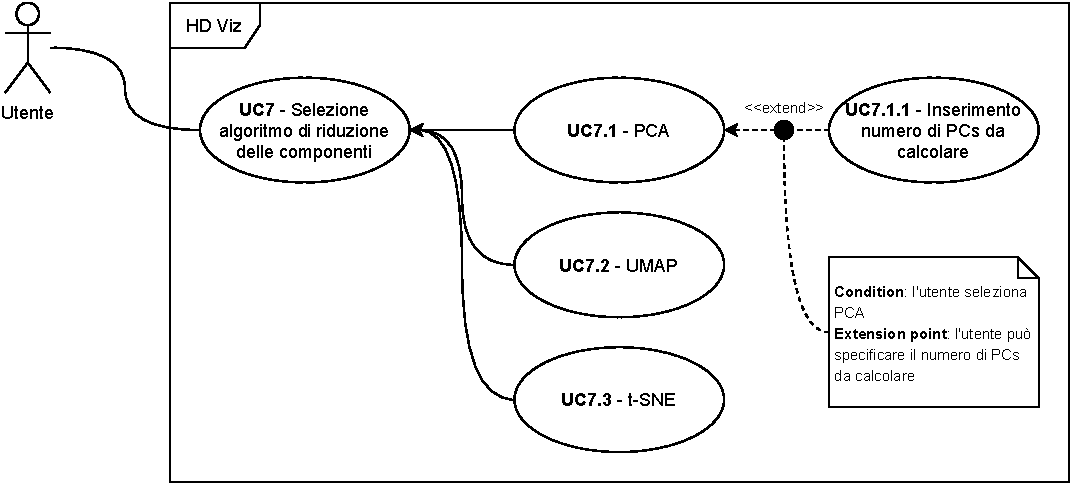
\includegraphics[width=0.9\textwidth]{source/sections/casi-uso/diagrams/uc7.pdf}
        \caption{UC7 - Selezione algoritmo di riduzione delle componenti}
        \label{fig:uc7}
    \end{figure}
    
    \begin{itemize}
    \item \textbf{Attore}: utente;
    \item \textbf{Descrizione}: l'utente sceglie l'algoritmo per la riduzione delle componenti per l'elaborazione dati;
    \item \textbf{Precondizione}: 
    \begin{itemize}
        \item eseguito l'upload del dataset come matrice $N\times M$ (\hyperref[uc1]{UC1});
        \item selezionato Linear Projection come visualizzazione \hyperref[uc2.5]{UC2.5}).
    \end{itemize}  
    \item \textbf{Postcondizione}: l'utente ha scelto l'algoritmo per la riduzione delle componenti;
    \item \textbf{Scenario Principale}: 
    \begin{enumerate}
        \item l'utente seleziona l'algoritmo per la riduzione delle componenti tra quelli disponibili.
    \end{enumerate}
    \item \textbf{Generalizzazioni}:
        \begin{enumerate}
            \item l'utente seleziona uno dei seguenti algoritmi di riduzione delle componenti:
                \begin{enumerate}
                    \item PCA (\hyperref[uc7.1]{UC7.1});
                    \item UMAP (\hyperref[uc7.2]{UC7.2});
                    \item t-SNE (\hyperref[uc7.3]{UC7.3}).
                \end{enumerate}
        \end{enumerate}  
    \end{itemize}
    
    \subsubsection{UC7.1 - PCA}
    \label{uc7.1}
    \begin{itemize}
    \item \textbf{Attore}: utente;
    \item \textbf{Descrizione}: il PCA è una tecnica di riduzione dimensionale, cioè a partire da $n$ features ne calcola $k$ ($k$ fissato), queste nuove k feature approssimano meglio le $n$ features iniziali;
    \item \textbf{Precondizione}: 
    \begin{itemize}
        \item eseguito l'upload del dataset come matrice $N\times M$ (\hyperref[uc1]{UC1});
        \item selezionato Linear Projection come visualizzazione (\hyperref[uc2.5]{UC2.5}).
    \end{itemize}  
    \item \textbf{Postcondizione}: il dataset contiene k nuove colonne (dove $k$ è il numero di PCs che l'utente ha scelto di calcolare), che sono le $k$ proiezioni calcolate da PCA;
    \item \textbf{Scenario Principale}: 
    \begin{enumerate}
        \item l'utente sceglie di applicare l'algoritmo PCA sul dataset.
    \end{enumerate}  
    \item \textbf{Inclusioni}:
        \begin{enumerate}
            \item inserimento del numero di PCs da calcolare (\hyperref[uc7.1.1]{UC7.1.1}).
        \end{enumerate} 
    \end{itemize}
    
    \paragraph{UC7.1.1 - PCA - Inserimento numero di PCs da calcolare}
    \label{uc7.1.1}
    \begin{itemize}
    \item \textbf{Attore}: utente;
    \item \textbf{Descrizione}: l'utente specifica quante nuove features il PCA deve calcolare;
    \item \textbf{Precondizione}: 
    \begin{itemize}
        \item eseguito l'upload del dataset come matrice $N\times M$ (\hyperref[uc1]{UC1});
        \item selezionato Linear Projection come visualizzazione (\hyperref[uc2.5]{UC2.5});
        \item selezionato PCA (\hyperref[uc7.1]{UC7.1}).
    \end{itemize}  
    \item \textbf{Postcondizione}: il numero k di features da calcolare è stato inserito;
    \item \textbf{Scenario Principale}: 
    \begin{enumerate}
        \item l'utente inserisce un numero k compreso tra 1 e il numero di features.
    \end{enumerate}  
    \end{itemize}
    
    \subsubsection{UC7.2 - UMAP}
    \label{uc7.2}
    \begin{itemize}
    \item \textbf{Attore}: utente;
    \item \textbf{Descrizione}: UMAP è una tecnica di riduzione dimensionale, cioè a partire da $n$ features ne calcola $k$ ($k$ fissato), queste nuove k feature approssimano meglio le $n$ features iniziali;
    \item \textbf{Precondizione}: 
    \begin{itemize}
        \item eseguito l'upload del dataset come matrice $N\times M$ (\hyperref[uc1]{UC1});
        \item selezionato Linear Projection come visualizzazione (\hyperref[uc2.5]{UC2.5}).
    \end{itemize}  
    \item \textbf{Postcondizione}: l'utente seleziona UMAP come algoritmo per la riduzione dimensionale;
    \item \textbf{Scenario Principale}: 
    \begin{enumerate}
        \item l'utente sceglie di applicare l'algoritmo UMAP sul dataset.
    \end{enumerate}
    \end{itemize}
    
    \subsubsection{UC7.3 - t-SNE}
    \label{uc7.3}
    \begin{itemize}
    \item \textbf{Attore}: utente;
    \item \textbf{Descrizione}: t-SNE è una tecnica di riduzione dimensionale, cioè a partire da $n$ features ne calcola $k$ ($k$ fissato), queste nuove k feature approssimano meglio le $n$ features iniziali;
    \item \textbf{Precondizione}: 
    \begin{itemize}
        \item eseguito l'upload del dataset come matrice $N\times M$ (\hyperref[uc1]{UC1});
        \item selezionato Linear Projection come visualizzazione (\hyperref[uc2.5]{UC2.5}).
    \end{itemize}  
    \item \textbf{Postcondizione}: l'utente seleziona t-SNE come algoritmo per la riduzione dimensionale;
    \item \textbf{Scenario Principale}: 
    \begin{enumerate}
        \item l'utente sceglie di applicare l'algoritmo t-SNE sul dataset.
    \end{enumerate}
    \end{itemize}
    
    
